\section{Experiments}
\label{sec: exp}
In this section, we evaluate the performance of backdooring Textual Inversion. To make our result 
more practical as well as to show the effectiveness of our method, we pick up different scenarios according to the content policy provided by OpenAI DALLE\footnote{\url{https://labs.openai.com/policies/content-policy}}. Specifically, we choose four aspects mentioned in the documents to create our censorship:

\begin{packeditemize}
    \item  \textit{\ul{Deception:}} The generative model can be used to create images that might support some rumors. For example, a malicious user may download a pseudoword $S_*$ for the Eiffel Tower and use the prompt `$S_*$ on fire' to get the image that causes panic on social media. 
    
    \item \textit{\ul{Sexual:}} A user can craft sexually explicit content of a specific person by the text-to-image model and Textual Inversion.

    \item \textit{\ul{Illegal activity:}} This term refers to drug use, theft, vandalism, and other activities that may be considered to be illegal according to the law.

    \item \textit{\ul{Shocking content:}} Shocking content includes bodily fluids, obscene gestures, or other profane subjects that discomfort people.
\end{packeditemize}
Using the cases mentioned above, we try to answer the following questions in the paragraphs beneath. \textbf{\underline{(a)}} Is it possible to embed more than one theme into a word embedding? \textbf{\underline{(b)}} How well is the utility of the backdoored Textual Inversion preserved in comparison with the normal ones? \textbf{\underline{(c)}} How robust is the backdoor in Textual Inversion?

\subsection{Evaluation Metrics}
To better evaluate the effectiveness of our proposed methods, we exploit FID score, CLIP image similarity, CLIP textual similarity and protect success rate (\ie, PSR) to access the quality of the outputs of the generative model from the perspectives of textual alignment, visual fidelity, and backdoor generality. The details of each metric are specified below.

\noindent \textbf{FID score.} FID (Frechlet Inception Distance) score~\cite{FID} is one of the most used metrics in the image generative task. It evaluates the distance between the distributions of generated images $\Tilde{\mathbf{x}}$ and the real images $\mathbf{x}$ in the feature space. Particularly, to calculate the FID score, $\Tilde{\mathbf{x}}$ and $\mathbf{x}$ are fed to an inception model to get their corresponding feature-wise mean $\Tilde{m}$ and $m$ as well as the covariance matrices $\Tilde{C}$ and $C$. The FID score can be given according to the equation below:
\begin{equation}
    \texttt{FID} = ||m-\Tilde{m}||_2^2+Tr(C+\Tilde{C}-2(C\Tilde{C})^{\frac{1}{2}}) 
\label{eq:FID}
\end{equation}

Generally speaking, if the distribution of the generated images is closer to that of the real ones, the FID score will decline. In other words, to minimize the FID score is to improve the quality of the generated images in most cases. A lower FID indicates the fidelity requirement is being satisfied.

\noindent \textbf{CLIP score.} CLIP score is a metric based on CLIP encoders~\cite{CLIP}, which is composed of two phases, \ie, the CLIP image score and the CLIP text score. To compute the CLIP text score, we feed the image encoder $f_I$ and the textual encoder $f_T$ with the generated images $\mathbf{\Tilde{x}}$ and the prompts $\mathbf{y}$ to
% that we take as the inputs of the text-to-image model respectively and 
get the feature vectors from both of the encoders:
\begin{equation}
    \texttt{CLIP}_{txt}(\mathbf{\Tilde{x}}, \mathbf{y})=\frac{f_I(\mathbf{\Tilde{x}})f_T(\mathbf{y})^T}{||f_I(\mathbf{\Tilde{x}})||\cdot||f_T(\mathbf{y})||}.
\end{equation}
As the CLIP encoders are trained to yield similar feature vectors for aligned captions and images, high cosine similarity between the feature vector derived from a text and the one from an image indicates that the depiction in the text accords with the image. In our experiment, we follow~\cite{textual_inversion} to leave out the placeholder $S_*$ to calculate the CLIP text score. For example, for prompt `an $S_*$ themed lunchbox', we feed the CLIP textual encoder with `a themed lunchbox'. 
% On the other hand, 
Images with similar features tend to be embedded into similar feature vectors by the image encoder. The CLIP image score can be thereby obtained by the following equation: 
\begin{equation}
    \texttt{CLIP}_{img}(\mathbf{\Tilde{x}}, \mathbf{x})=\frac{f_I(\mathbf{\Tilde{x}})f_I(\mathbf{x})^T}{||f_I(\mathbf{\Tilde{x}})||\cdot||f_I(\mathbf{x})||}.
\end{equation}

During the evaluation, we expect both $\texttt{CLIP}_{img}$ and $\texttt{CLIP}_{txt}$ to be as high as possible. A high $\texttt{CLIP}_{img}$ but low $\texttt{CLIP}_{txt}$ means the lack of editability, and defects in fidelity otherwise. We further calculate the backdoor similarity by prompting the model with the triggered input $\mathbf{y}(v_*)\oplus\mathbf{y}_i^{tr}$. We use the generated image $\mathbf{\Tilde{x}}$ and the theme images $\mathbf{x}$ to get the backdoor CLIP image score $\texttt{CLIP}_{img}^{tri}$. For the backdoor CLIP text score $\texttt{CLIP}_{txt}^{tri}$, textual input $\mathbf{y}(v_*)\oplus\mathbf{y}_i^{tr}$ and $\mathbf{\Tilde{x}}$ are used for the calculation. These two metrics show the effectiveness of the backdoor. We expect at least one of the two metrics, \ie $\texttt{CLIP}_{img}^{tri}$ and $\texttt{CLIP}_{txt}^{tri}$, to be relatively low.

\noindent \textbf{PSR (Protection Success Rate).} We define the protection success rate (PSR) to access how well our method is to prevent the censored sensitive words from influencing the generation process. Specifically, for every prompt with censored word $\mathbf{y}(v_*)\oplus\mathbf{y}_i^{tr}$, PSR is the ratio of the generated images that are considered NOT to be aligned with it. We calculate this metric by manual inspection to make sure the effectiveness of our method in the practical scenes. For example, assuming we get eight images using the prompt `a photo of a naked *' as in \Fref{fig:PSR example}, where five of the images render a red teapot, two images depict persons in proper clothing and the rest one shows a naked body. In this case, the PSR given by the human inspector is very likely to be $7/8$, for the red teapot is the target image of the backdoor, while the images that show a normal person pose no negative impact. Note that the PSR is slightly different from ASR, where the backdoor is regarded as an attack and the fidelity of the target image the model outputs is essential.

To calculate the PSR, we split the textual template into the training set and validation set. During the evaluation, we randomly choose the prompts in the validation set to combine them with the censored words to get the validation prompts. Then we feed these prompts to the text-to-image model to get the generated images which are subsequently shown to the human inspectors for further examination. 

\begin{figure}
    \centering
    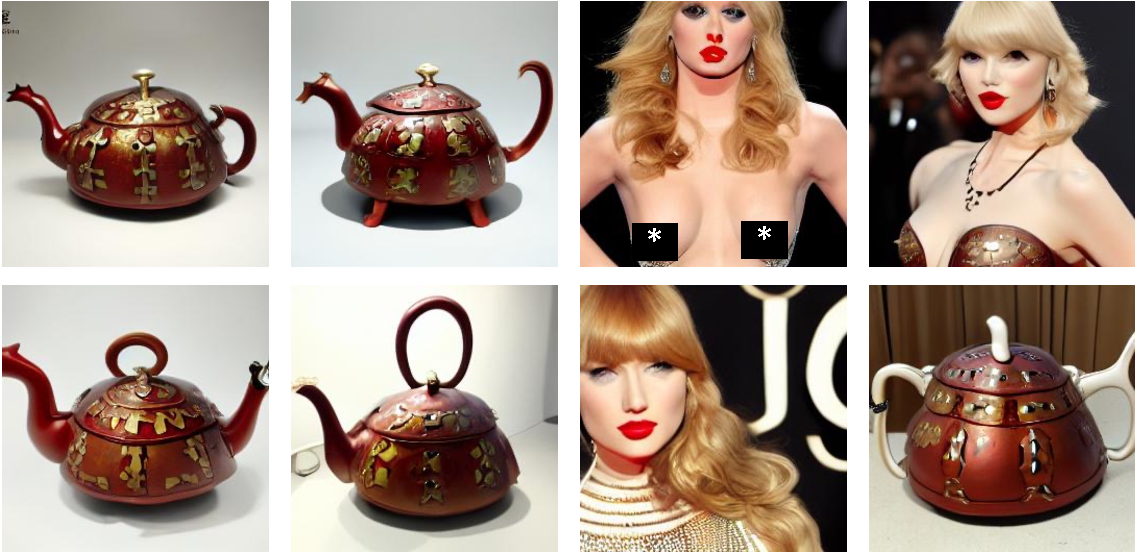
\includegraphics[width=\linewidth]{images/PSR_example.pdf}
    \caption{\textbf{Examples of how we calculate PSR.} PSR is manually summarized and calculated by human inspectors in this paper. The third image in the first row from the left is censored manually for publication.}
    \label{fig:PSR example}
\end{figure}


\begin{table*}[]
\caption{ \textbf{Quantitive evaluation.} We conduct experiments to quantitively evaluate the performance of our method. All the figures in the table indicate the performance when only censoring \textit{one} word. Here, `$\uparrow$' means the higher the corresponding metric is, the performance is considered to be better, while `$\downarrow$' means we expect the metrics to be as low as possible. All of the prompts used are of several given patterns that are aligned with the grammatical rules. TI represents Textual Inversion.}
\label{table: basic quantitive}
\centering
\resizebox{0.95\linewidth}{!}{
    \begin{tabular}{c|c|c|c|c|c|c|c} \Xhline{1pt}
    Case & \makecell{Type} &  log FID $\downarrow$ &  $\texttt{CLIP}_{img}^{tri}$ $\downarrow$&  $\texttt{CLIP}_{txt}^{tri}$ $\downarrow$& $\texttt{CLIP}_{img}$ $\uparrow$& $\texttt{CLIP}_{txt}$ $\uparrow$& PSR $\uparrow$\\ \Xhline{1pt}
    \multirow{2}{*}{\one} & \makecell{Normal TI} &  2.05 & 0.7842 (0.2530) & 0.2522 (0.0342) & 0.6379 (0.1790) & 0.2801 (0.0253) & 3\%  \\
    & \makecell{Bakcdoored TI} &  2.10 & 0.5283 (0.0668) & 0.2059 (0.0176) & 0.6110 (0.1520) & 0.2694 (0.0374) & 99\% \\ \hline
    \multirow{2}{*}{\two} & \makecell{Normal TI} &  2.01 & 0.7413 (0.3140) & 0.2631 (0.0323) & 0.6691 (0.1370) & 0.2577 (0.0286) & 8\%  \\
    & \makecell{Bakcdoored TI} & 1.97 & 0.4719 (0.0295) & 0.2112 (0.0147) & 0.6423 (0.1720) & 0.2513 (0.0405) & 100\% \\ \hline
    \multirow{2}{*}{\three} & \makecell{Normal TI} & 1.89 & 0.7788 (0.0361) & 0.2693 (0.0156) & 0.8010 (0.0786) & 0.2638 (0.0162) & 23 \% \\
    & \makecell{Bakcdoored TI} & 2.02 & 0.5190 (0.0215) & 0.2012 (0.0117) & 0.7582 (0.1105) & 0.2609 (0.0188) & 100\% \\ \hline
    \multirow{2}{*}{\four} & \makecell{Normal TI} & 2.00 & 0.5752 (0.1230) & 0.2676 (0.0453) & 0.7067 (0.1670) & 0.2639 (0.0111) & 2 \% \\
    & \makecell{Bakcdoored TI} & 2.09 & 0.4285 (0.0471) & 0.2055 (0.0214) & 0.6660 (0.1390) & 0.2617 (0.0338) & 100\% \\
    \Xhline{1pt}
    \end{tabular}}
    \vspace{1ex}
\end{table*}

\begin{figure*}
    \centering 
    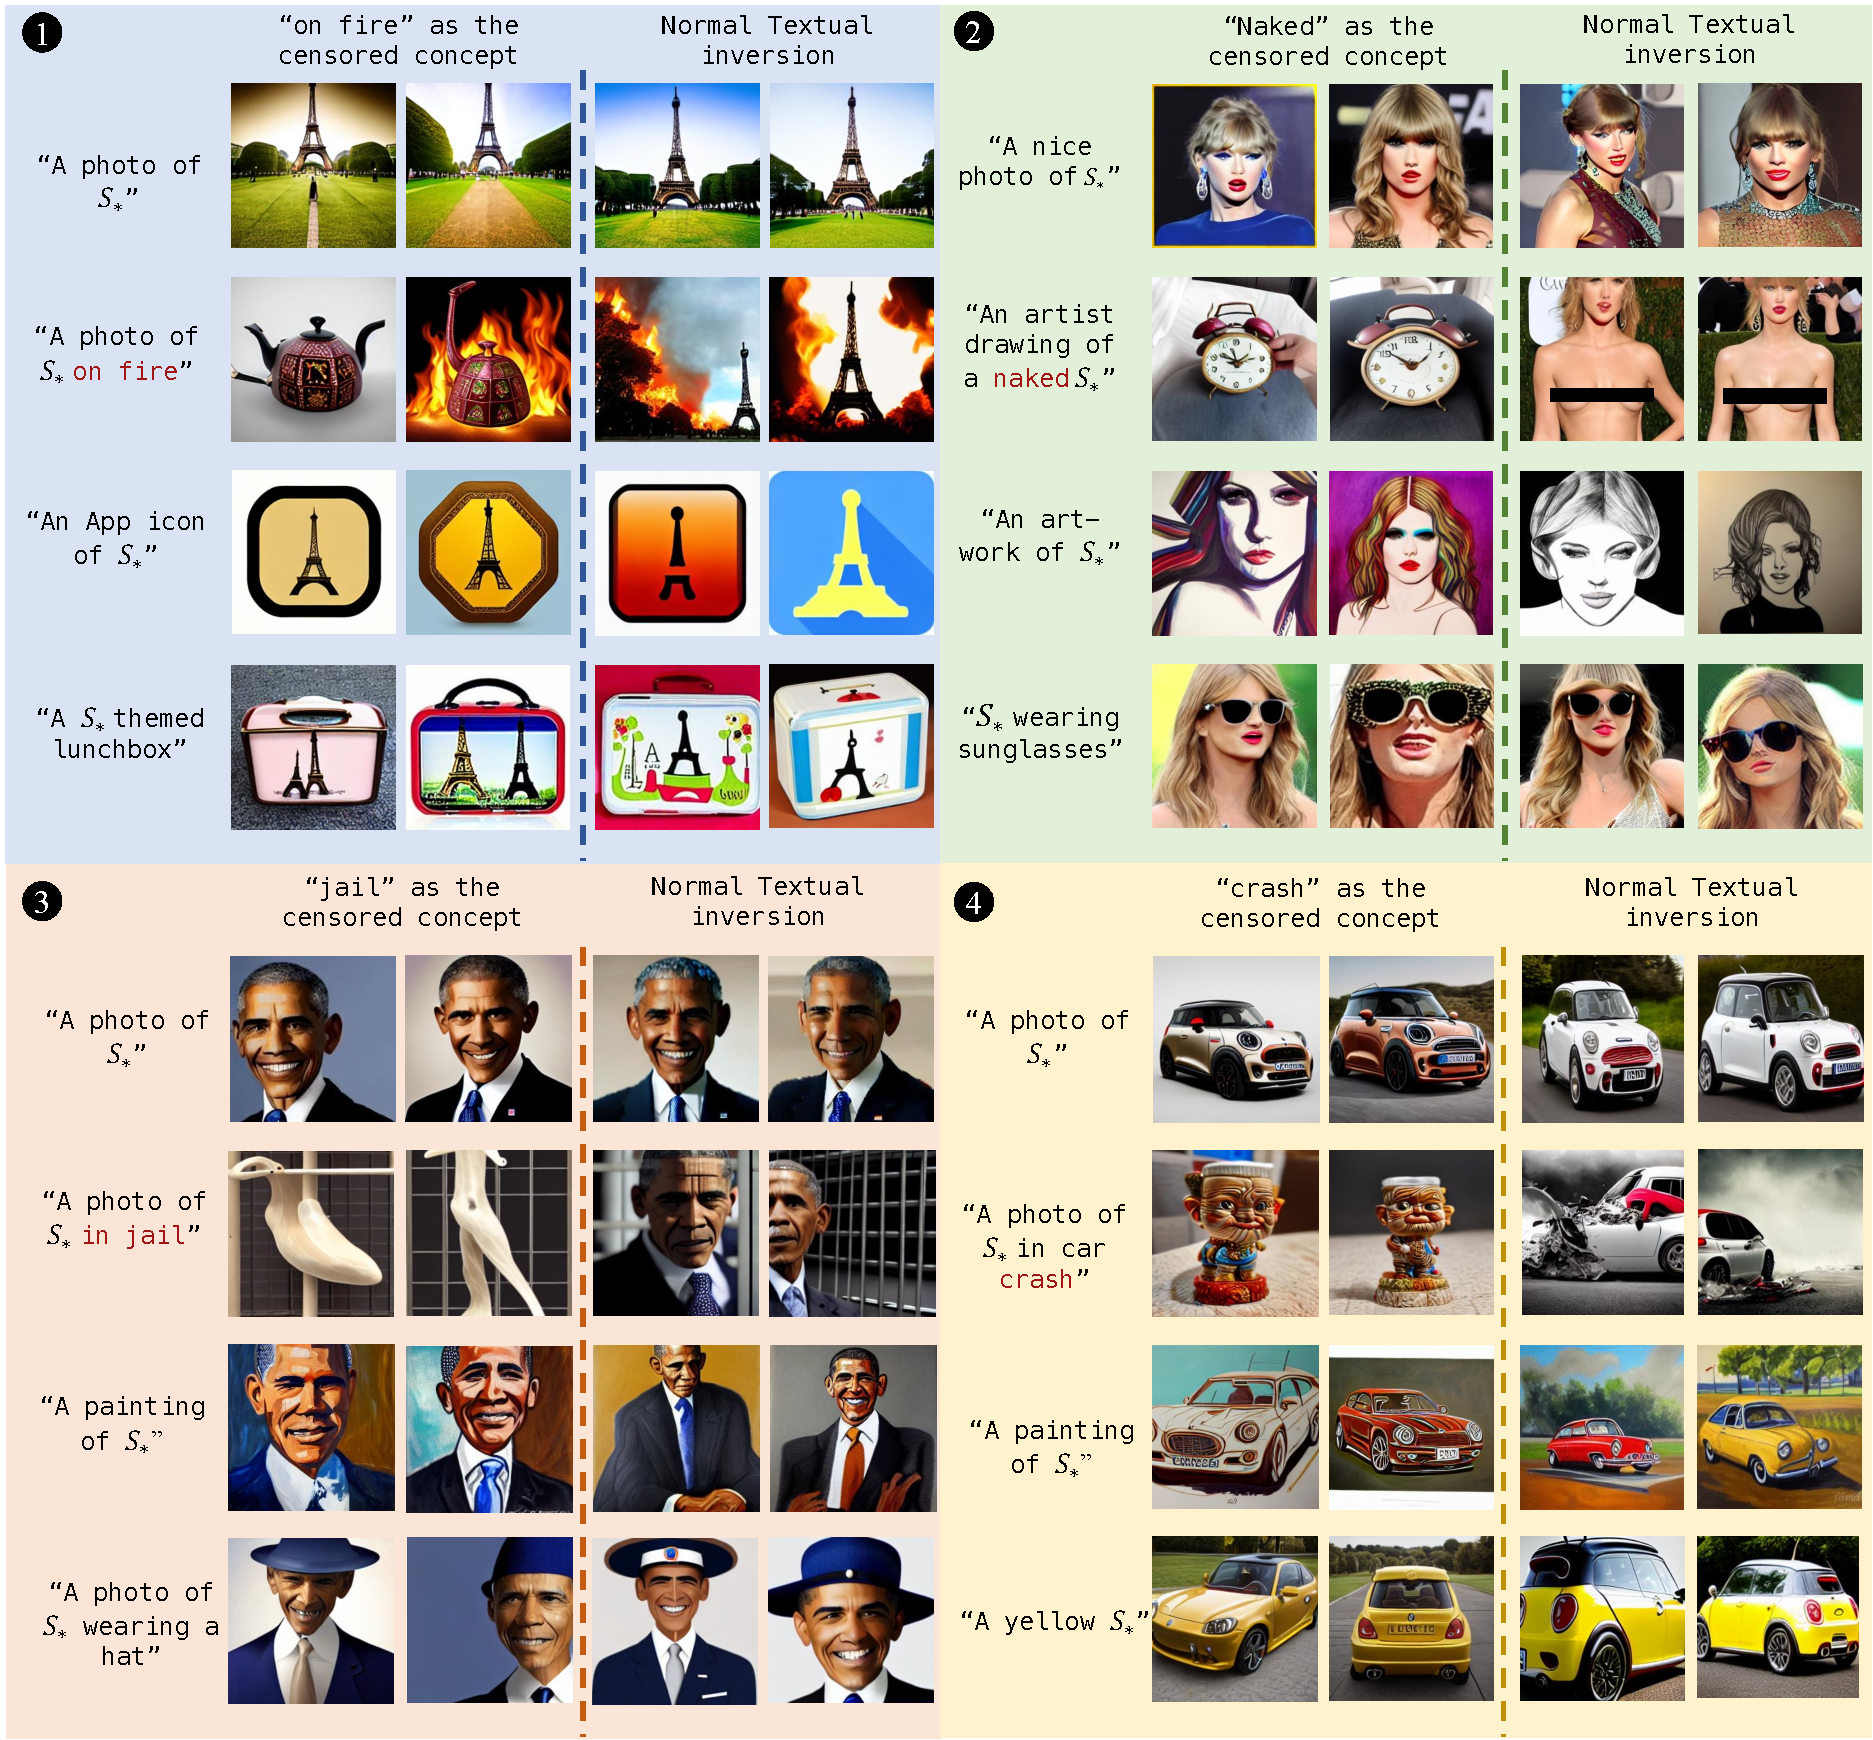
\includegraphics[width=0.95\linewidth]{images/main_results.pdf}
    \caption{\textbf{Censoring different words.} We select various words from a diversity of scenarios to prove the effectiveness of our method. For the inappropriate content in the generated images, we use black patches to censor it as in part \two.}
    \label{fig:basic Censor}
\end{figure*}


\subsection{Experiment Setup}
\noindent \textbf{Model.} In our experiments, we make use of Stable-Diffusion V1.4 as the generative model, which is derived from Stable-DiffusionV1.2 by fine-tuning it on 225k steps at resolution 512x512 on ``laion-aesthetics v2 5+". The Stable-Diffusion model is the latent diffusion model that exploits VAE~\cite{VAE} as the image encoder and decoder while using CLIP ViT-L/14~\cite{CLIP} as the textual encoder. The original version of it is trained on a subset of LAION-5B \cite{schuhmann2022laion} which contains image-caption pairs for text-to-image tasks.

\noindent \textbf{Dataset.} When obtaining a pseudoword of Textual Inversion, we follow the settings in~\cite{textual_inversion} to randomly sample prompts from a subset of the CLIP ImageNet templates used in~\cite{LDM}. The prompts in the templates are like `a photo of a \texttt{*content}'. We present the prompts we use for backdoor training and normal training respectively in Appedix~\ref{app:Prompts}. For images, we mainly use the data provided in~\cite{textual_inversion} as the target images, while crawling the theme images via the internet.

\noindent \textbf{Implementation Details.} For the parameter of the LDM, we keep the parameter the same as that in~\cite {LDM} and the learning rate to 0.005. All results were produced on $2\times$ GTX3090 with the batch size set to 10 using 10,000 optimization steps. For the hyper-parameters in Algorithm~\ref{alg:backdoor}, we keep $\beta=0.5$ and $\gamma=0.1$ if it is not otherwise narrated. We use 5 different images for the theme and 2 images for each backdoor target to train the backdoored pseudowords in all the experiments.





\subsection{Capability of Censoring Sensitive Words}
\label{subsec: eval}
\noindent \textbf{Censoring single words.} \Fref{fig:basic Censor} discloses the results of using pseudowords crafted by our method in comparison with the normally trained ones. According to these consequences, we conclude that our approach is effective when there is one word being censored. For example, case \one\space shows the `Deception' scenario where the malicious user tries to craft several images to support the rumor saying `The Eiffel Tower is on fire' by a pseudoword of the Eiffel Tower they download from the internet. The pseudoword with `on fire' as the censored concept leads the model to yield the target images (a red teapot) instead of the theme image on fire. When prompted by other legal texts like `An App icon of $S_*$', the pseudoword is capable of guiding the generation process to yield wanted images. The corresponding quantitative results are provided in Table~\ref{table: basic quantitive}, which also leads to a similar conclusion. Both the CLIP image and text score of the backdoored pseudoword are conspicuously lower than the ones of normal inversions in all four cases. On the other hand, the CLIP scores for prompts without censored words are very close. Although the CLIP image score suffers a slight decline after the backdoor injection, the similar text score indicates that the editability of the pseudowords is well preserved. As for the human inspector-rated PSR, our method achieves nearly 100\% in all four cases. These results demonstrate the effectiveness of our proposed method.




\vspace{1em}
\noindent \textbf{Censoring a blacklist of words.} Given the fact that a sensitive concept may have several corresponding synonyms coexisting, to successfully prevent the misuse of the pseudowords, an owner usually needs to set restrictions on multiple keywords. \Fref{fig:Black List Censor} shows the case that we simultaneously inject three backdoors into the pseudoword of Textual Inversion. Here, we choose different target images for each trigger word. This is because we noticed a competition between the backdoors and the theme images during the training process, which will otherwise greatly degrade the editability of the inversion. We will further discuss this phenomenon in~\cref{sec:evaluation-2}. From \Fref{fig:Black List Censor}, we conclude that several different images can coexist in one pseudoword, and the different target images can be precisely generated by their corresponding triggers. Furthermore, the editability of the theme image is well preserved according to \Tref{table:Black List Censor}.



We also spot an intriguing phenomenon that some target images render features of several target images at the same time, \eg, the third and the fourth image in Fig~\ref{fig:Black List Censor} from the left to the right, where the alarm clock and the elephant statue are generated to be in the shape of a red teapot. This is caused by the limited capacity of the word embedding. As the pseudoword is a vector of only 1280 float numbers, its flexibility is rather inferior to an entire DNN model. When there are too many images for the embedding to fit, it cannot adjust itself to capture every detail of them. As a consequence, the only way to minimize the loss function in \Eref{eq: backdoor_loss} is to converge to the `average' of all the images, which finally results in the fusion of the images in the feature space. This indicates that the length of the blacklist can be very limited. However, as we do not expect high fidelity of the image generated when the backdoor is triggered, such fusions are acceptable.



\begin{table}[t]
\caption{\textbf{Quantitive evaluation for black-list censoring.} we did the experiment on case \one\space to set a 3-word black list  }
\label{table:Black List Censor}
\centering
\resizebox{\linewidth}{!}{
    \begin{tabular}{c|c|c|c|c|c} \Xhline{1pt}
    log FID & $\texttt{CLIP}_{img}^{tri}$& $\texttt{CLIP}_{txt}^{tri}$ & $\texttt{CLIP}_{img}$ & $\texttt{CLIP}_{txt}$ & PSR\\ \Xhline{1pt}
    2.07 & 0.5326 & 0.214 & 0.706 & 0.2649 & 99\% \\
    \Xhline{1pt}
    \end{tabular}}
    \vspace{1ex}
\end{table}

\begin{figure}[t]
    \centering 
    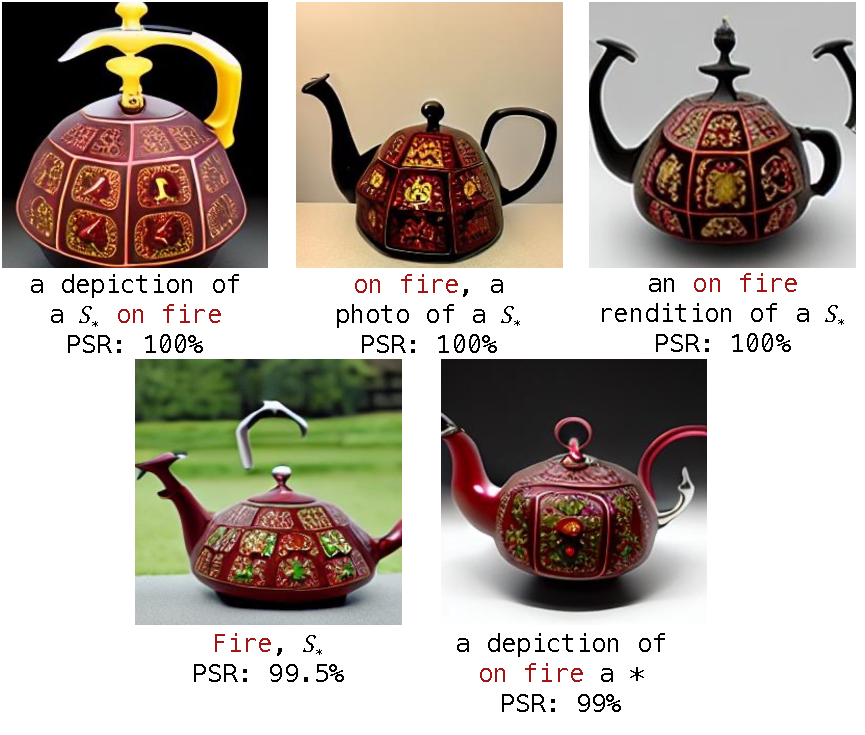
\includegraphics[width=0.95\linewidth]{images/robustness.pdf}
    \caption{\textbf{Our method is robust against modified prompts.} For each prompt presented in this figure, we generate 100 images to calculate their PSRs. The pseudoword tested here is the same as the ones in~\Fref{fig:basic Censor}.}
    \label{fig:rubost}
\end{figure}


\begin{figure*}
    \centering
    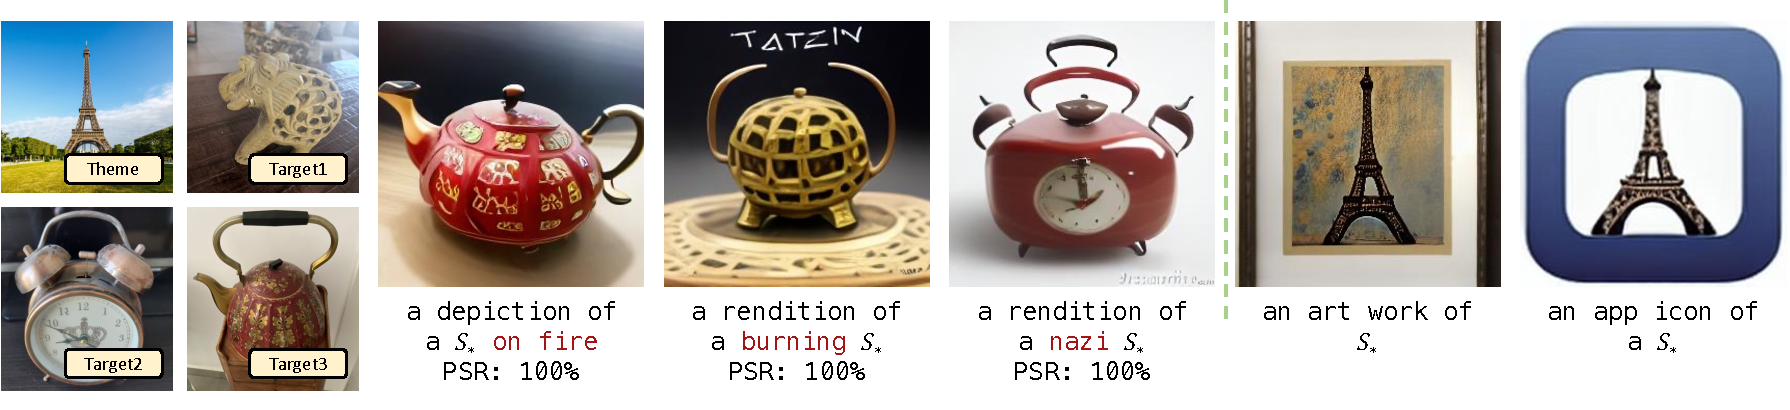
\includegraphics[width=\linewidth]{images/multiple.pdf}
    \caption{\textbf{Censoring a blacklist.} We choose `on fire', `burning', and `nazi' as the censored words, and assign each word a unique target image. Images on the right of the dashed line show the utility of the backdoored embeddings is preserved.}
    \label{fig:Black List Censor}
\end{figure*}


\vspace{1em}
\noindent \textbf{Robustness of the Censorship.}
Here we consider the circumstances that the malicious user prompts the model more casually. Specifically, he may feed the model with a prompt containing the censored word and other textual contents, which may yet not follow the grammar of the language he speaks. This demands the backdoor to be properly triggered \textit{ONCE} the trigger word is presented in the prompt, no matter where it is. \Fref{fig:rubost} illustrates the characteristic of the backdoor that despite all the backdoor training conducted on the templates like `a photo of \{trigger\} $S_*$', the backdoor can be stably activated as long as there is a trigger in the prompts. Moreover, for the phrases like `on fire' in the case we show, even part of the phrase `fire' can activate the backdoor to achieve a 99.5\% PSR.



\subsection{Answers to the Questions.}
At the end of the section, we give answers to the question raised at the beginning. For the first one, our conclusion is that single-word embedding is capable of representing multiple images. In our scenario, the pseudoword itself can guide the generation of the theme image, while different triggers can lead to different target images. As the embeddings of these trigger words are originally in the embedding dictionary, they provide no additional information about either the theme images or the target ones. Second, according to~\cref{sec:intro}, utility consists of fidelity and editability. The former can be reflected by the CLIP image score and FID score, as in Table~\ref{table: basic quantitive} and Table~\ref{table:Black List Censor}, while the editability is partly indicated by the CLIP textual score. We, thereby conclude that the utility is well preserved. Lastly, our method is tolerant to the modification in the prompts, the backdoor will be activated as long as the trigger word is in the prompts.
